\documentclass[a0paper,portrait]{baposter}
\usepackage{amsmath,amssymb,amsthm} 
\newtheorem{theorem}{Theorem}[section]

% Auxiliary commands
\DeclareMathSymbol{:}{\mathpunct}{operators}{"3A}%semicolon spaces
\RequirePackage{xspace}
\def\mat#1{\ensuremath{#1}\xspace}
\def\dmat#1#2{\gdef#1{\mat{#2}}}
\def\csdmat#1#2{\csdef{#1}{\mat{#2}}}

% Define some abbreviations that we can use later
\def\lh{\lambda h}  % Shorthand for lambda h

% Define the custom \term command for highlighting terms
\newcommand{\term}[1]{\textcolor{blue}{\textit{#1}}} % blue italics
\newcommand{\Lim}[1]{\raisebox{0.5ex}{\scalebox{0.8}{$\displaystyle \lim_{#1}\;$}}}

% Mathbb Letters. Usage: \bA
\def\defbb#1{\csdmat{b#1}{\mathbb{#1}}}
\forcsvlist\defbb{A,B,C,D,E,F,G,H,I,J,K,L,M,N,O,P,Q,R,S,T,U,V,W,X,Y,Z}
\RequirePackage{bbm}
\dmat\bk{\mathbbm k}

% Mathcal Letters. Usage: \cA
\def\defcal#1{\csdmat{c#1}{\mathcal{#1}}}
\forcsvlist\defcal{A,B,C,D,E,F,G,H,I,J,K,L,M,N,O,P,Q,R,S,T,U,V,W,X,Y,Z}

% Structures
\def\set#1{\left\{#1\right\}}
\def\sets#1#2{\left\{\left.#1\ \right\vert#2\right\}}
\def\rbr#1{\left(#1\right)}
\def\ang#1{\left\langle#1\right\rangle}
\def\n#1{\left\lvert#1\right\rvert}
\def\nn#1{\left\lVert#1\right\rVert}

\usepackage{lipsum}
\usepackage{multicol}
\usepackage[colorlinks, linkcolor=black, urlcolor=black, citecolor=black]{hyperref} % hyperreferences with black links


\newtheorem{theorem*}{Theorem}
\definecolor{lightblue}{rgb}{0.1,0.46,0.72}
\definecolor{blue}{rgb}{0.1,0.46,1}

\graphicspath{{../Graphs}}

\begin{document}

\begin{poster}
{
columns=2,
headerborder=closed, % Adds a border around the header of content boxes
bgColorOne=white, % Background color for the gradient on the left side of the poster
bgColorTwo=white, % Background color for the gradient on the right side of the poster
boxColorOne=white, % Background color of the content boxes
headerColorOne=lightblue, % Background color for the header in the content boxes (left side)
headerColorTwo=lightblue, % Background color for the header in the content boxes (right side)
borderColor=lightblue, % Border color
headerFontColor=white, % Text color for the header text in the content boxes
textborder=rounded, % Format of the border around content boxes, can be: none, bars, coils, triangles, rectangle, rounded, roundedsmall, roundedright or faded
%eyecatcher=1, % Set to false for ignoring the left logo in the title and move the title left
headershape=rounded, % Specify the rounded corner in the content box headers, can be: rectangle, small-rounded, roundedright, roundedleft or rounded
}
{}%left logo
{The\; Stability\; of\; Complex\; Time\; Steppers}
{\medskip\textsc{Cian J. Duggan}}
{\includegraphics[width=6cm]{trinity-stacked.jpg}}

\headerbox{Introduction}{name=intro,column=0,row=0}{
This poster looks at the stability of numerical methods when applied to problems of differential calculus.\\ This project aims to add a visual understanding to the concepts of stability. It also aims to explore the use of complex time steps in numerical methods.\\
}
\headerbox{Key Terminology}{name=box1,column=0,below=intro}{
\textbf{Numerical Methods} are iterative algorithms used to approximate solutions to problems that cannot be solved exactly.\\
These methods are often employed to solve differential equations.\\

\par The infinitesimal $h$ in $y'(t) = \Lim{h \to 0} \frac{y(t+h) - y(t)}{h}$ cannot be represented on a computer.\\
Instead, a finite \textbf{time step} $h$ is used to approximate the derivative.\\

\par A numerical method is \textbf{stable} for a given size of time step if the solution does not diverge from the exact solution.\\
The choice of step size is crucial; too large, and the solution will diverge, too small, and the solution will cost computational resources.\\

\par Shown below is \textbf{Runge-Kutta 4} applied to the Exponential Decay Problem.\\
The exact solution is known, and shown in black.\\
Stable and unstable choices of $h$ are shown in green and red respectively.\\
\begin{center}
\includegraphics[width=0.95\textwidth]{Exponential Decay/Exact vs Method/Runge-Kutta 4 real.png}
\end{center}
}

\headerbox{The Exponential Decay Problem}{name=box2,column=0,below=box1}{
Consider a quantity $y$ that decays relative to its current value.\\
The quantity at time $t$ is $y(t)$.\\
The rate of decay is $\lambda \in \bC$ with $Re(\lambda) < 0$.\\
The simplest case of this problem is described by the differential equation:\\
$y'(t) = \lambda y(t) \quad \text{with} \quad y(0) = 1$\\
This has the exact solution $y(t) = e^{\lambda t}$ giving the name \textit{Exponential Decay}.\\
\begin{center}
\includegraphics[width=0.7\textwidth]{Exponential Decay/Exact with (-0.3+5j).png}
\end{center}
}

\headerbox{Stability}{name=box3,column=1}{%,aligned=intro}{
We can define the \textbf{Stability Function} $s(\lambda, h)$ for any numerical method by writing the algorithm in the form $y_{j+1} = s(\lambda, h) y_{j}$.\\
A method is stable for any pair in $S = \{ (\lambda, h) : |s(\lambda, h)| < 1\} \in \bC$, the \textbf{Stability Region}.\\
Applying \textbf{Runge-Kutta 4}: $y_{j+1} = (1 + \lh + \frac{{(\lh)}^2}{2} + \frac{{(\lh)}^3}{6} + \frac{{(\lh)}^4}{24})y_j$
\vspace{0.3cm}
\begin{multicols}{2}
The stability function is\\
$s(\lambda, h) = \sum\limits_{n=0}^{4}\frac{{(\lh)}^n}{n!}$\\
$S$ is shown on the right.\\
S is divided into subregions,\\ 
each corresponding to a different\\
range of $|s(\lambda, h)|$ values.\\
The methods with these step sizes are shown below, for $\lambda \in \bR^{-}$:
\columnbreak{}
\vspace*{-1.1cm}
\begin{center}
\includegraphics[width=0.45\textwidth]{Stability Magnitude/Color/Runge-Kutta 4.png}
\end{center}
\end{multicols}
\vspace{-0.5cm}
\begin{center}
\includegraphics[width=0.9\textwidth]{Stability Magnitude/Exponential Decay/Runge-Kutta 4.png}
\end{center}
}
\headerbox{The Complex Domain}{name=box4,column=1,below=box3}{
It has often proven useful to extend the analysis of a problem to the complex domain. We will have a look at the stability of numerical methods when the chosen time-step is complex.\\
\vspace{-0.75cm}
\begin{multicols}{2}
We want to take an overall step of size $h \in \bR$ comprised of two steps $z_1, z_2 \in \bC$ such that $z_1 + z_2 = h$.\\
We compare to the case where we take $2$ steps of size $\frac{h}{2} \in \bR$.\\
The following diagram shows the case\\
$z_1 = \frac{h}{2}(1+i)$ and $z_2 = \bar{z_1}$
\columnbreak{}
\vspace*{0.05cm}
\begin{center}
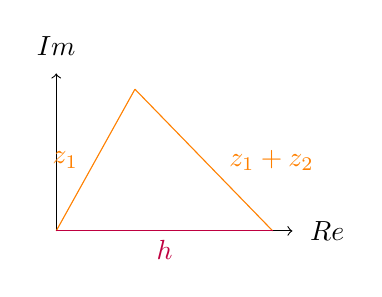
\begin{tikzpicture}
	\draw[->] (0,0) -- (3,0) node[right, shift={(0.1, 0)}] {$Re$};
	\draw[->] (0,0) -- (0,2) node[above, shift={(0,0.1)}] {$Im$};
	\draw[-, color=orange] (0,0) -- (1,1.8) node[midway, shift={(-0.1,0)}, left] {$z_1$};
	\draw[-, color=orange] (1,1.8) -- (2.75,0) node[midway, shift={(0.2,0)}, right] {$z_1 + z_2$};
	\draw[color=purple] (0,0) -- (2.75,0) node[midway, below] {$h$};
\end{tikzpicture}
\end{center}
\end{multicols}
\begin{multicols}{2}
\vspace*{-0.9cm}
\begin{center}
\includegraphics[width=0.49\textwidth]{Stability Regions/Graphs/Real VS Complex Comparison/Runge-Kutta 4.png}
\end{center}
\columnbreak{}
\vspace*{0.1cm}
\textit{George, Yung and Mangan}\cite{walking_into_the_complex_domain} show that the error is reduced when using complex time steps.\\
For Runge-Kutta 4, we obtain two different stability functions\\
$s_{_{\bR}}(\lambda, h)$ and $s_{_{\bC}}(\lambda, h)$\\
They give the stability regions shown on the left.\\
While the error may decrease, the stability region decreases with it.
\end{multicols}
}


\headerbox{References}{name=refer,column=1,below=box4}{
\vspace{-0.5cm}
\providecommand{\bysame}{\leavevmode\hbox to3em{\hrulefill}\thinspace}
\providecommand{\href}[2]{#2}
\renewcommand\refname{} % Remove the title "References" from the bibliography
\begin{thebibliography}{1}

\bibitem{walking_into_the_complex_domain}
Jithin D. George, Samuel Y. Jung, and Niall M. Mangan,\\
\emph{{W}alking into the complex plane to `order' better time integrators}, 2021.\\
\url{https://arxiv.org/abs/2110.04402}
\bibitem{GitHub_Repo}
The GitHub repository for this project,\\
\url{https://github.com/CianJDuggan/Capstone-Project}

\end{thebibliography}

}

\end{poster}

\end{document}
